\section{Vision}

\subsection{Requirements}
You'll need the following python packages to successfully run the vision:

\begin{description}
\item \texttt{Polygon2} Polygon is a python package that handles polygonal shapes in 2D. 
\item \texttt{argparse} Python command-line parsing library
\item \texttt{pyserial} Python Serial Port Extension
\item \texttt{numpy} Array processing for numbers, strings, records, and objects.
\item \texttt{openCV} OpenCV-Python is the Python API of OpenCV. It combines the best qualities of OpenCV C++ API and Python language.
\end{description}

To install them run these commands in the terminal:

\shellcmd{pip install --user Polygon2==2.0.6} \\
\shellcmd{pip install --user argparse==1.3.0} \\
\shellcmd{pip install --user pyserial==2.7} \\
\shellcmd{pip install --user numpy}  

You can also learn how to install openCV from the following link:
\url{http://docs.opencv.org/2.4/doc/tutorials/introduction/linux_install/linux_install.html}

\subsection{Usage}
Before using the vision system, you can look at the vision feed by typing \texttt{xawtv} in the command prompt. This will launch only the vision feed, where you can experiment with the different settings.

In order to launch the vision system:
\begin{itemize}
\item Run the main vision file: \texttt{python vision.py}
\item At first, a window for the automatic colour calibration will pop out. You'll need to follow the instructions as printed in the terminal. 
\item The calibration goes through all the colours that are used for the vision (\texttt{red}, \texttt{yellow}, \texttt{blue}, \texttt{green}, \texttt{pink}) and requires \textbf{multiple clicks for each} one of them to get their thresholds properly.
\item You need to press the \texttt{q} key after each calibrated colour. 
\item If you want to skip the calibration you can simply press the \texttt{Esc} key and the vision will use the previously saved calibrations.
\item The vision processing will then be launched.
\end{itemize}

\subsection{Graphic Interface}
There will be a window labelled \texttt{Filter output}, where presenting the vision feed after all filters have been applied to the original. This output is overlayed with icons representing the robots and the ball, if they are found (see \autoref{fig:pitch}). Robots are represented by an inner circle of the team colour (\texttt{yellow} or \texttt{blue}), an outer circle identifying which of the two team members it is (\texttt{pink} or \texttt{green}) and an arrow oriented in the direction of the robot.  The red ball is displayed by drawing a red circle around where it was detected. 

\begin{figure}[H]
\centering
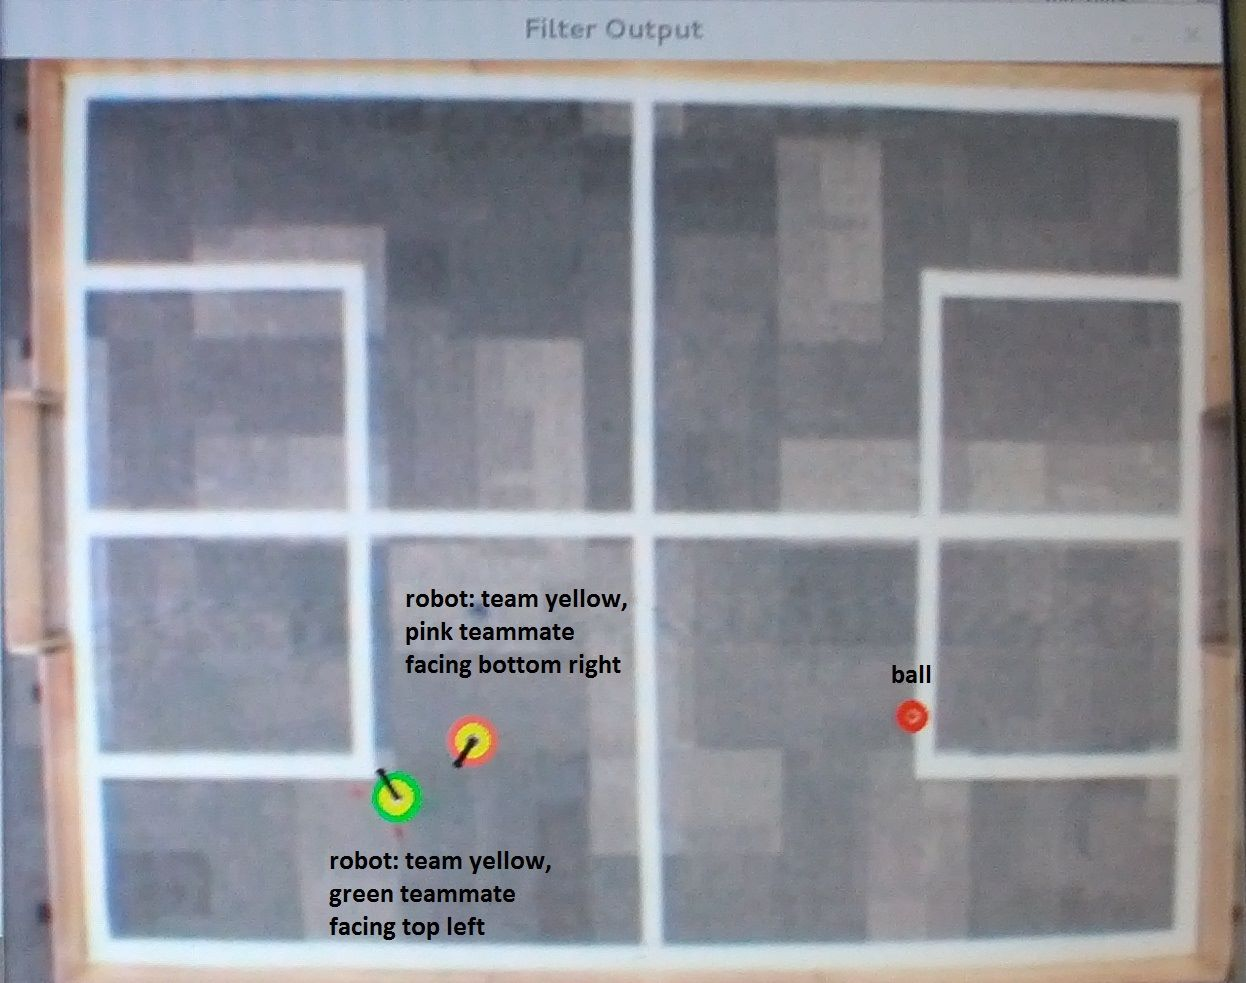
\includegraphics[scale=0.2]{vision_pitch}
\caption{Vision Frame with Overlay}
\label{fig:pitch}
\end{figure}

There are two other windows containing several sliders for filters that that can be applied to the feed (see \autoref{fig:filters}) and more advanced options for specific filters (see \autoref{fig:params}). The set of filters available includes masks for specific colours, a manually configurable colour mask, and apply different effects to the frame.



\begin{figure}[H]
\centering
\begin{subfigure}{.5\textwidth}
\centering
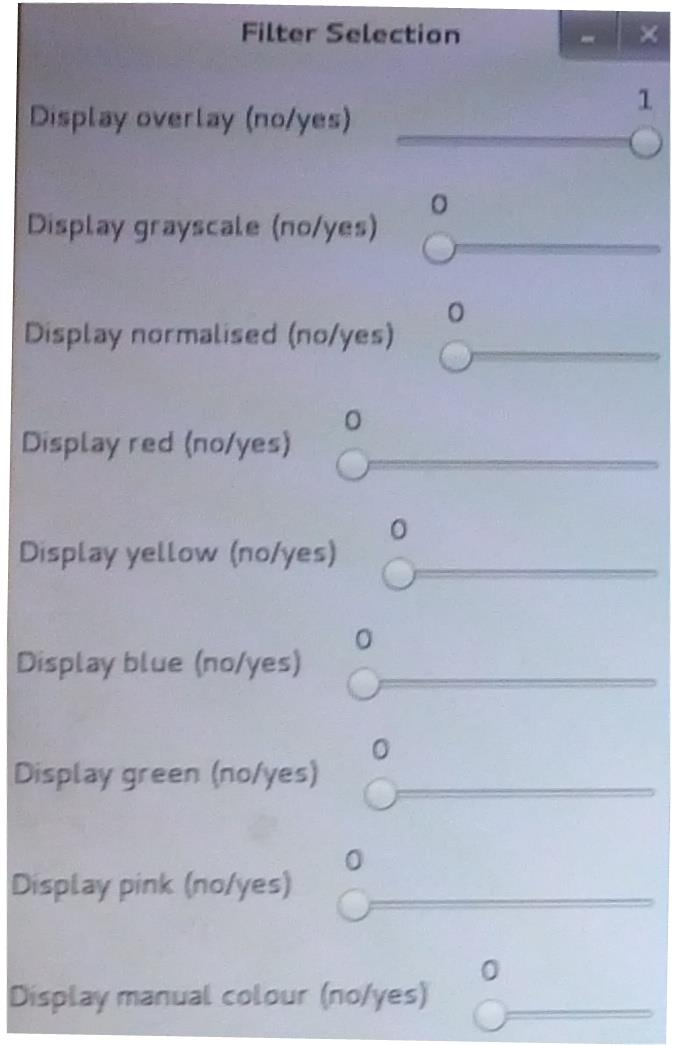
\includegraphics[scale=0.2]{vision_filters}
\caption{Available Filters}
\label{fig:filters}
\end{subfigure}%
\begin{subfigure}{.5\textwidth}
\centering
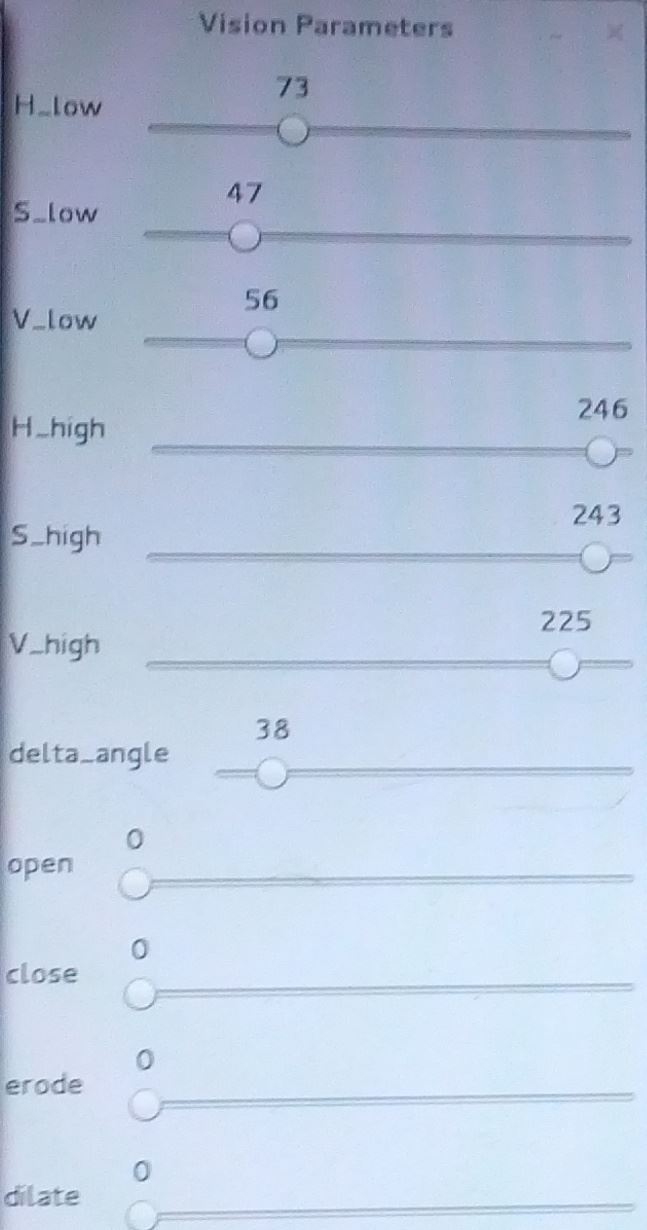
\includegraphics[scale=0.2]{vision_params}
\caption{Advanced Filter Parameters}
\label{fig:params}
\end{subfigure}
\caption{GUI Controls}
\label{fig:sliders}
\end{figure}





When the vision is running, it outputs the coordinates of all found objects, their orientation and velocity relative to the previous taken frame. These objects are returned as a dictionary and passed to the planner. This is achieved by passing a callback method for updating the planner world model when initialising the vision module. This method is called on every vision frame parsed, and it ensures the planner has the latest data.
